The current version of analysis defines the BDT regions in \twocentral channel such that sufficient \zjets{} events are present in each region. If we could have better \zjets{} modelling, a more Higgs sensitive definition of BDT regions could be achieved and could improve the analysis. The following is an example of such a BDT definition.  To define the first region in the \twocentral channel we choose the top 30\% VBF signal to ensure that the \Mbb{} distribution is well-behaved in the low-mass sideband as the BDT score correlation with\ Mbb{} is non-linear for very high BDT scores. (See Appendix~\ref{sec:app-bdt} for details on the correlation between \Mbb, BDT score and \pTbb).  To select the remaining regions we scan the VBF signal events in the lower 70\% of  BDT scores and maximize the sum of $\frac{S}{\sqrt{B}}$ in the Higgs mass window (100~\GeV$<\Mbb<$140~\GeV). The definition of the signal regions, the yields of each processes and the estimation of sensitivity are listed in Tables~\ref{tab:BDTReg2cen_sensitive}. The MC templates and parametrization of signal are shown in Figures~\ref{fig:sigpar_sensitive}. The $\chi^2$ between simulated and fitted distributions are summarized in Table~\ref{tab:sigpar_sensitive}. 

The non-resonant background for this definition of BDT regions (shown in Fig. \ref{fig:mbb_sidebands_sensitive}) is estimated the same way as the main analysis. The $\chi^2$ test, F-test and spurious signal test are summarized in Tables. \ref{tab:chi2-2cen_sensitive} \ref{tab:f-test_sensitive} and \ref{tab:spurious-test-2cen_sensitive}. We choose Bernstein O2 polynomial for SR I and Bernstein O3 polynomial for all other regions for \twocentral channel. The toy experiments results of the combined channel fit are presented in Fig. \ref{fig:MCToy_sensitive}. The Asimov fit yields the uncertainty $\Delta \mu_{H} = 1.40$ and the corresponding \zjets{} sensitivities of each channel are summarized in Table. \ref{tab:zstrength_sensitive}. 

This definition of BDT regions has limited constraining power of the \zjets{} components in the mosted sensitive regions, SR I of \twocentral channel for instance. We performed a side-band only fit to extract \zjets{} contribution independently in all regions. The fitted \zjets{} strengths are summarized in Table. \ref{tab:zsidebandfit_sensitive}. The effective $\mu_{Z}$ of all regioins combined is $1.03\pm 0.52$ in the sideband only fit with a compatibility of $\chi^2/nodf = 13.56/8=1.70$ ($\chi^2$ probability of 9.4\%). The concern of this BDT definition is that the low constraining power of \zjets{} may yield potential bias of the $\mu_{H}$ value as shown in Fig. \ref{fig:SRI_overlay_sensitive}. For the main analysis, since we adopt the strategy that allows sufficient \zjets{} events to be present in all regions of the \twocentral channel, we observed that the analytical functions we picked have consistent description of the non-resonant background within the Higgs mass window as shown in Fig. \ref{fig:2cen_overlay} and \ref{fig:4cen_overlay}.

\begin{table}[htbp]
\centering
\caption{A more Higgs sensitive signal region definitions, yields and sensitivities for the \twocentral channel. }
\label{tab:BDTReg2cen_sensitive}
\begin{tabular}{|l|l|l|l|l|}
\hline
Region                       & SR I                & SR II                      & SR III                      & SR IV                 \\ \hline
BDT Score Range              & \textgreater0.046   & [0.021, 0.046]             & [-0.009, 0.021]             & \textless-0.021       \\ \hline
\multicolumn{5}{|c|}{Total Yield}                                                                                                     \\ \hline
QCD $Z$                      & $50.78 \pm 18.50$   & $214.69 \pm 42.00$         & $791.42 \pm 82.92$          & $1340.35 \pm 100.9$   \\ \cline{2-5} 
EWK $Z$                      & $15.96 \pm 1.09$    & $22.41 \pm 1.35$         & $37.56 \pm 1.73$            & $49.64\pm 1.90$       \\ \hline
\multicolumn{5}{|c|}{Sideband}                                                                                                        \\ \hline
Non-res. (sideband low)  & $1781 \pm 42.20$    & $5594 \pm 74.79 $          & $18409 \pm 135.68$          & $59791 \pm 244.52$    \\ \cline{2-5} 
Non-res. (sideband high) & $2974 \pm 54.53$    & $9659 \pm 98.28 $          & $30343 \pm 174.19$          & $96258 \pm 310.25$    \\ \hline
\multicolumn{5}{|c|}{Yield in Higgs Mass Window}                                                                                      \\ \hline
VBF                          & $40.50 \pm 0.48$    & $33.35\pm 0.40$            & $29.97\pm 0.36$             & $19.68 \pm 0.24$      \\ \cline{2-5} 
ggF                          & $3.13 \pm 0.10$     & $5.61\pm 0.18$             & $5.38\pm 0.17$              & $68.93 \pm 2.18$      \\ \cline{2-5} 
No-res.(extrapolated)   & $2466.82 \pm 49.67$ & $7976.18 \pm 89.31$        & $26974.94\pm 164.24$        & $87827.61 \pm 296.36$ \\ \hline
\multicolumn{5}{|c|}{Expected Sensitivity}                                                                                            \\ \hline
$S/ \sqrt(B)$                & 0.88                & 0.44                       & 0.31                        & 0.29                  \\ \hline
\end{tabular}
\end{table} 


\begin{figure}[htbp]
  \centering    
 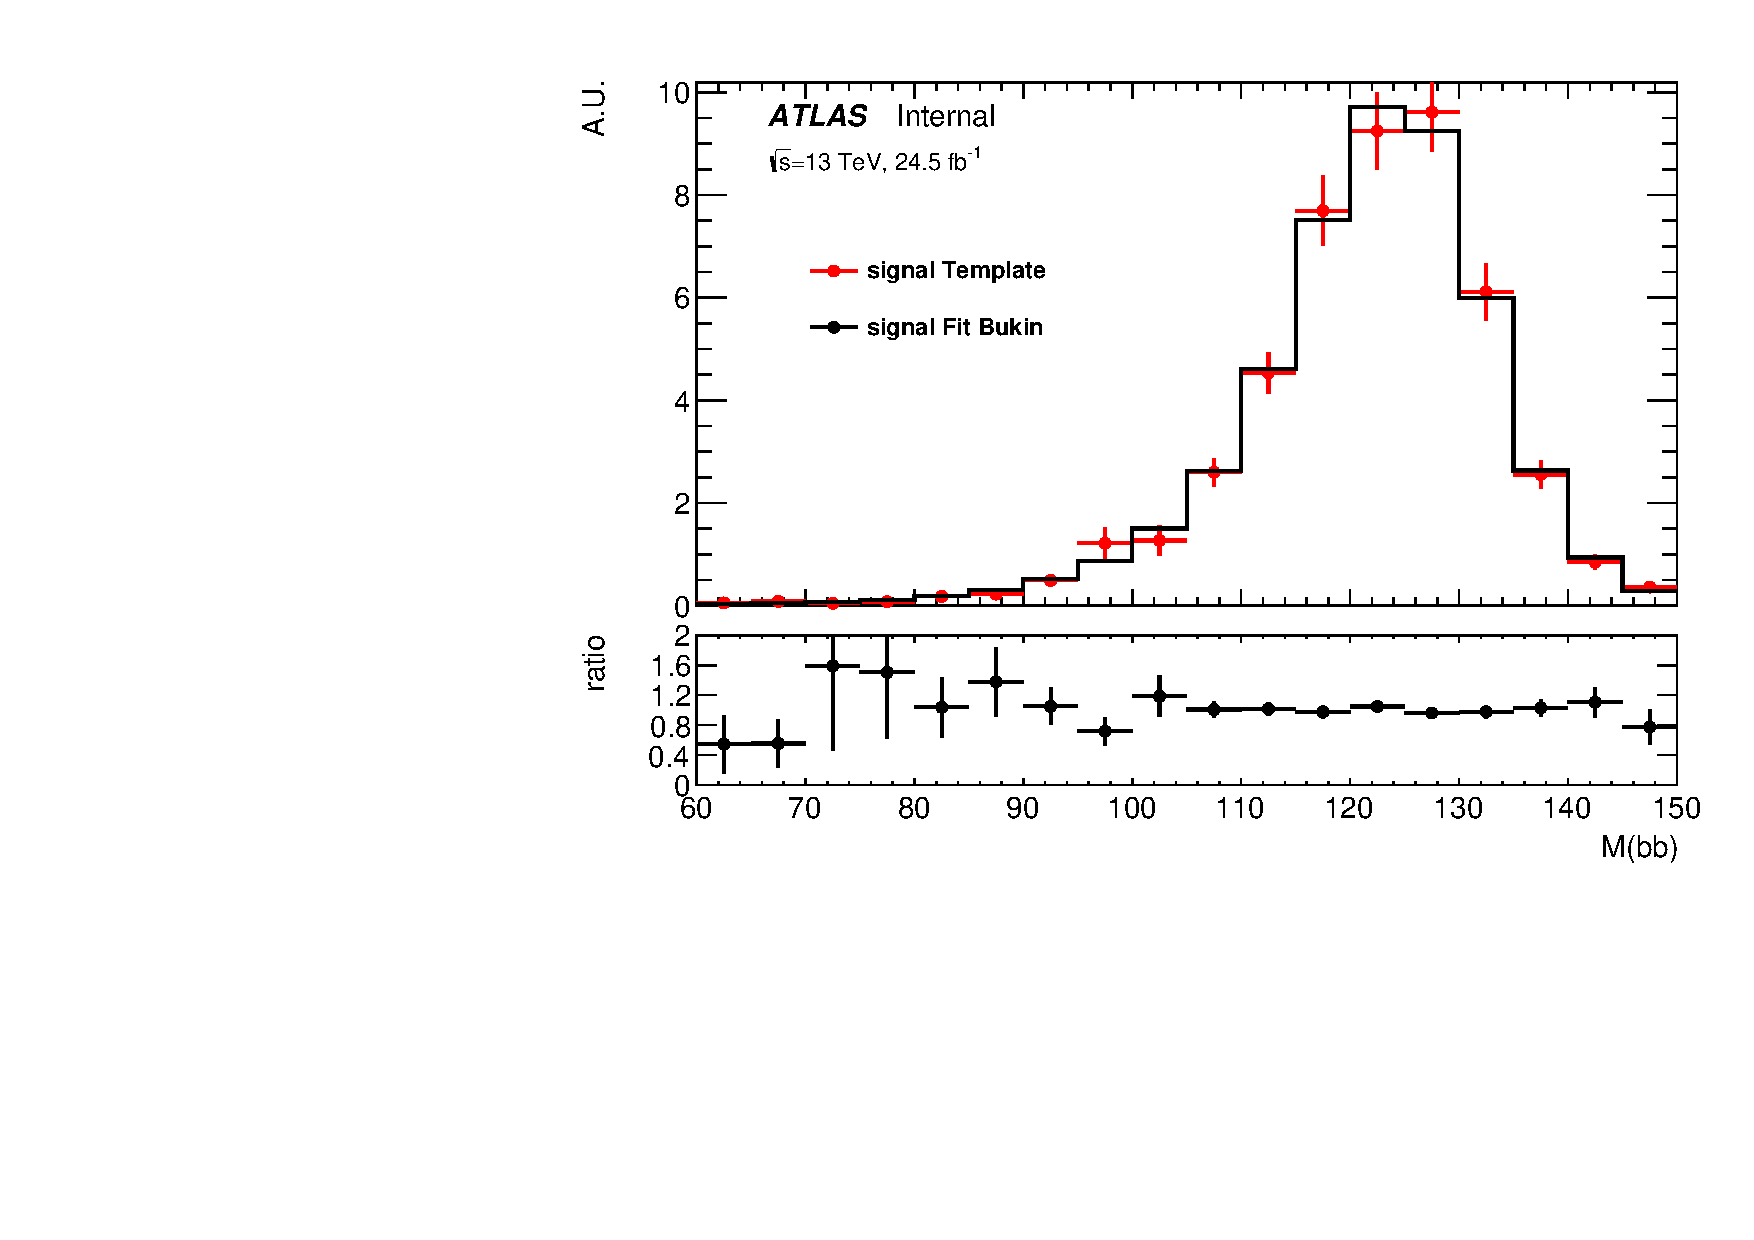
\includegraphics[width=0.24\textwidth]{figures_alt/sig_2cen_SRI.pdf}
 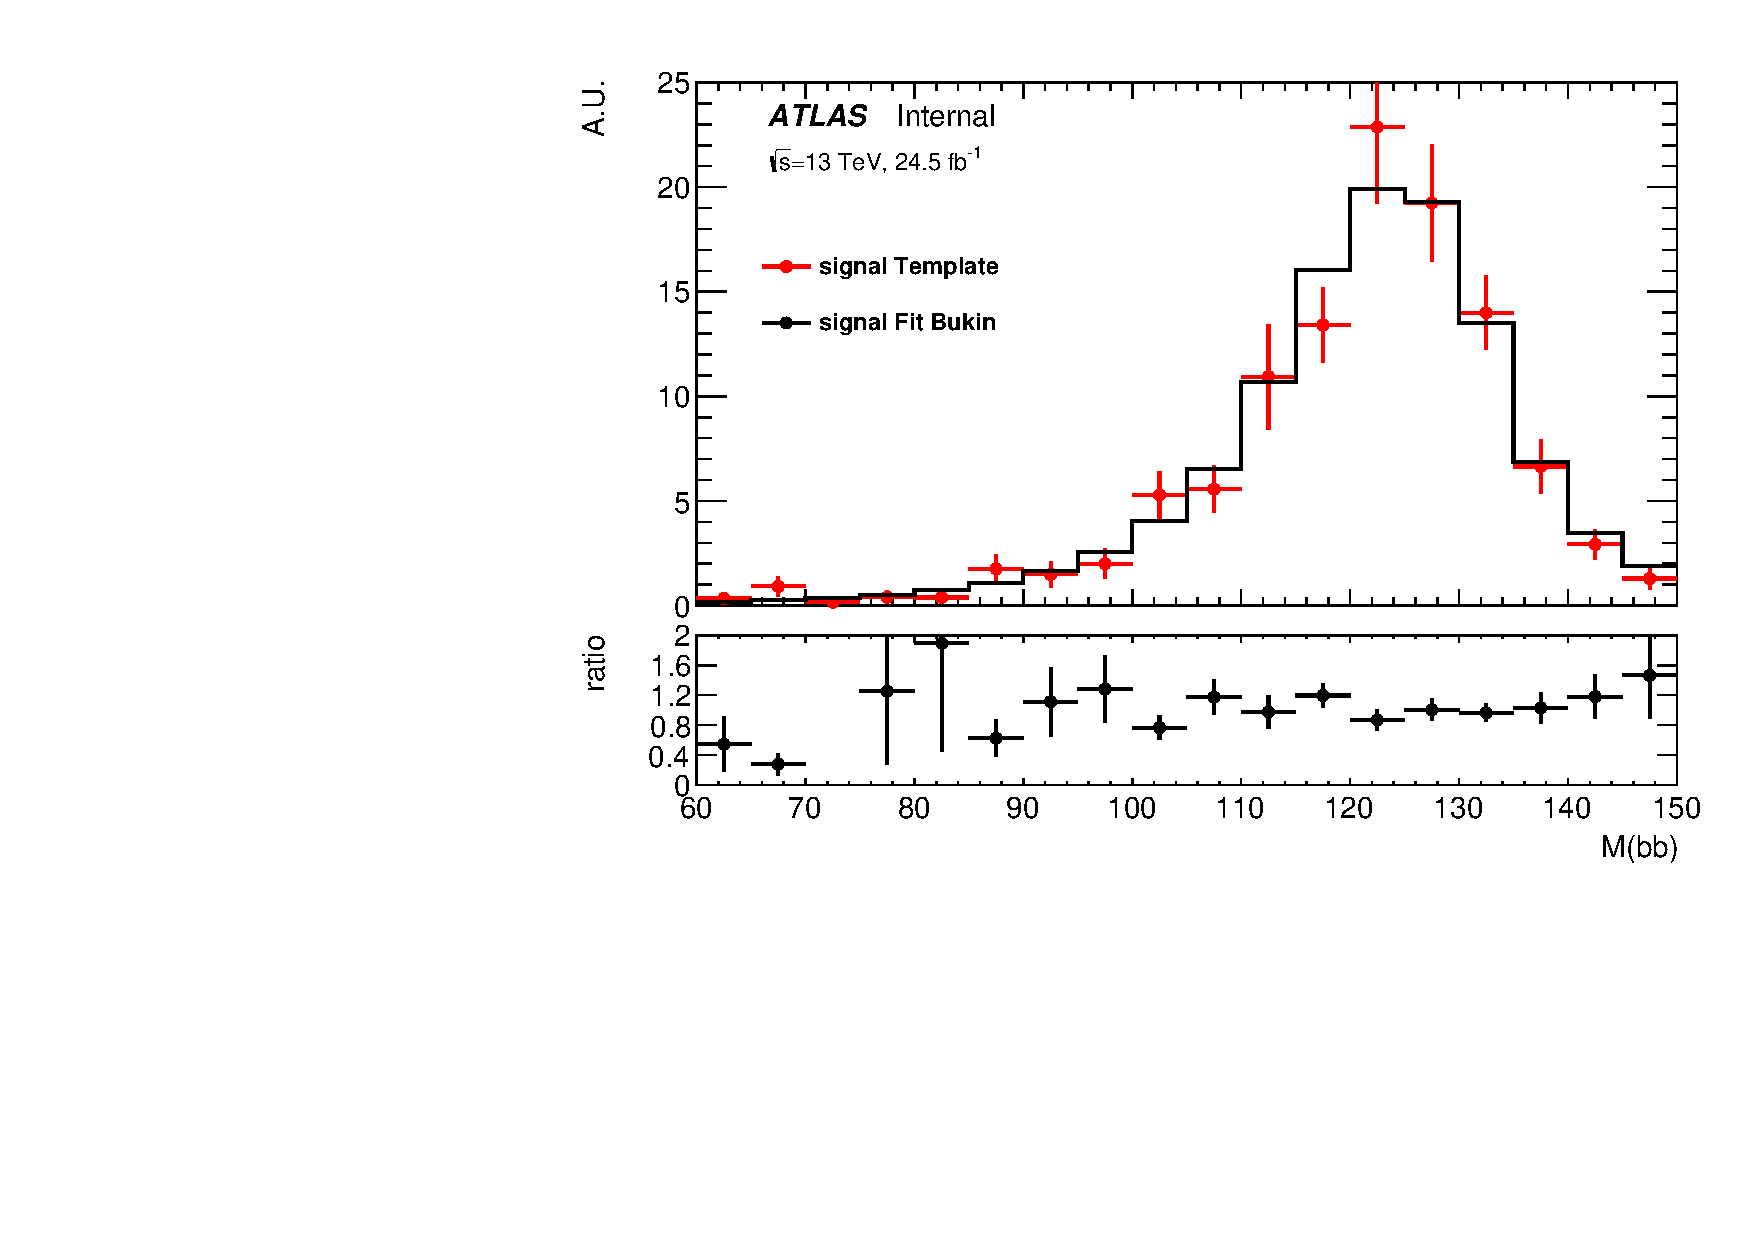
\includegraphics[width=0.24\textwidth]{figures_alt/sig_2cen_SRII.pdf}
 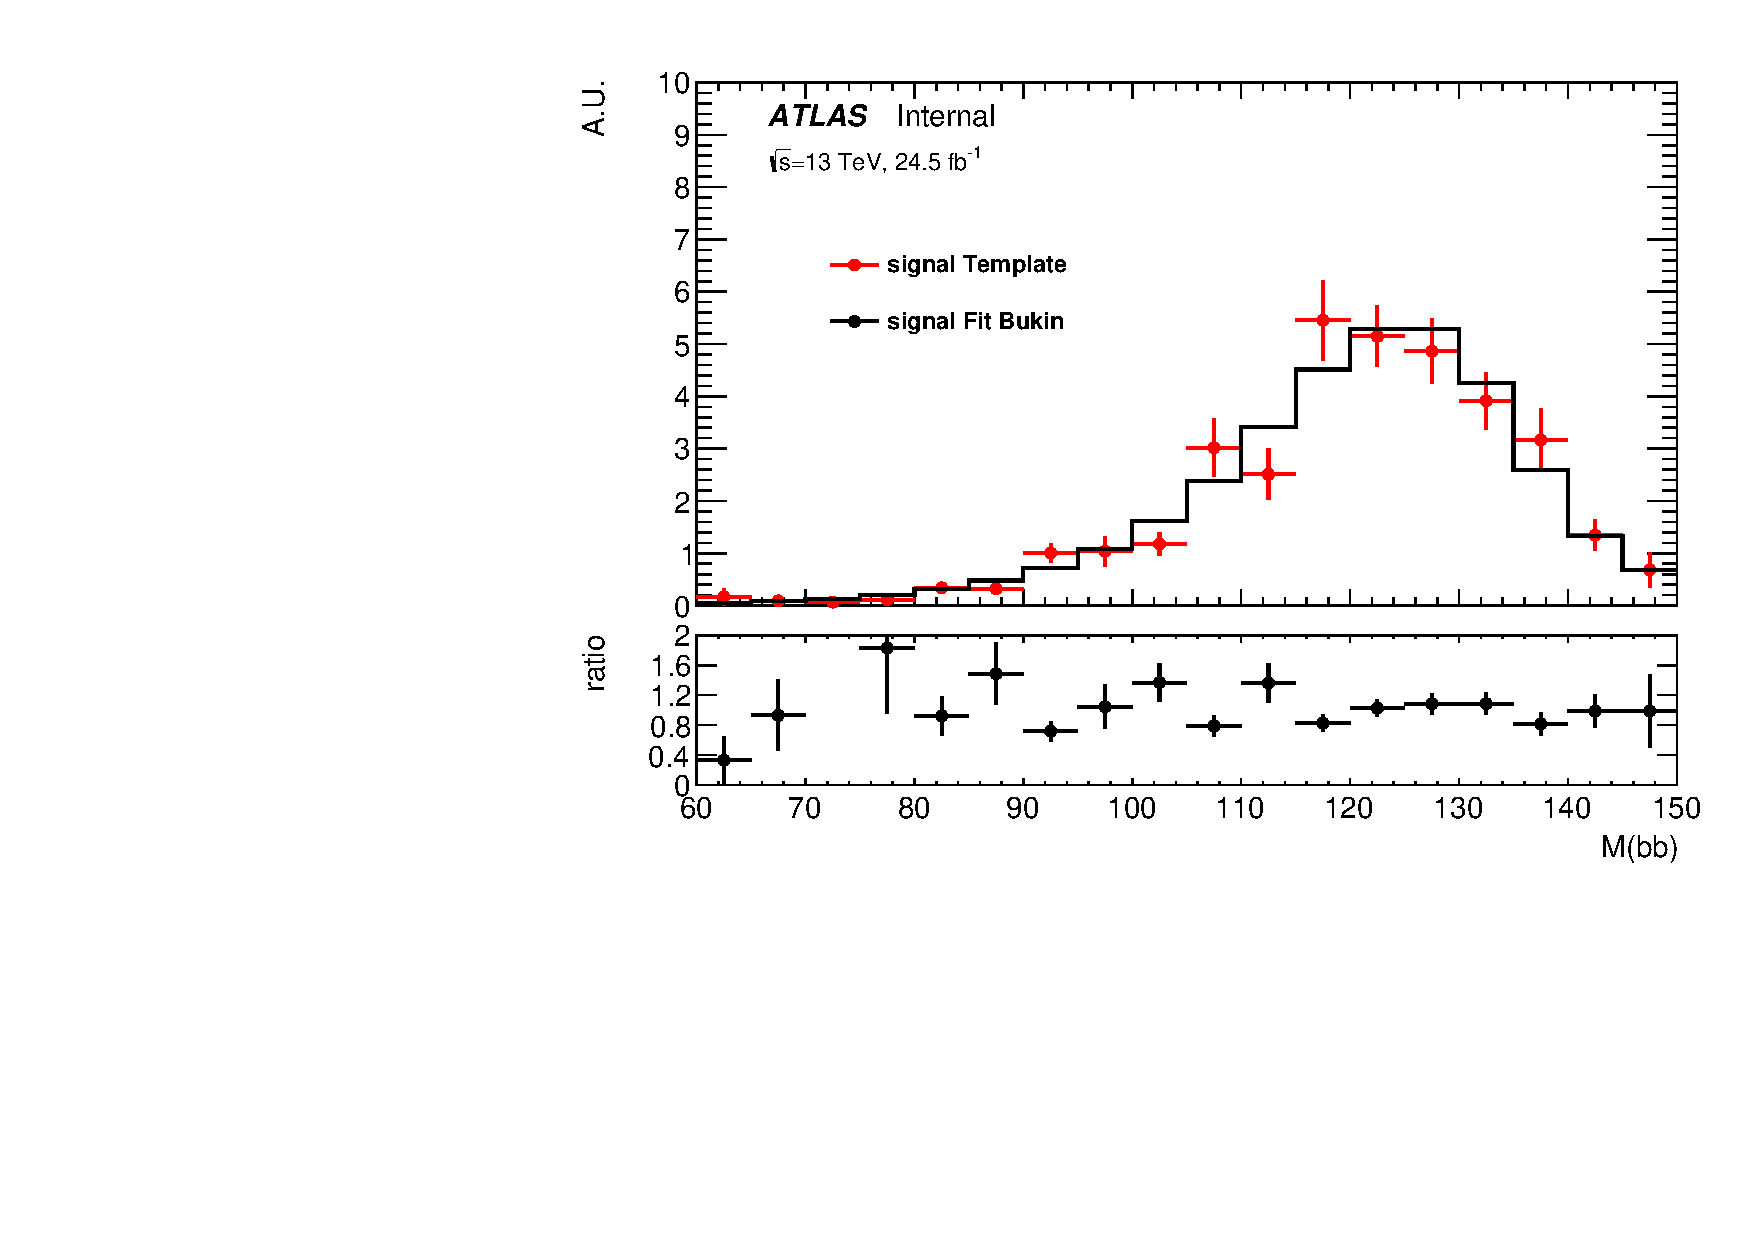
\includegraphics[width=0.24\textwidth]{figures_alt/sig_2cen_SRIII.pdf}
 \includegraphics[width=0.24\textwidth]{figures_alt/sig_2cen_SRIIV.pdf}

\caption{Bukin function parametrization of signal \Mbb{} distributions of SR I to SR IV (left to right) in \twocentral}
  \label{fig:sigpar_sensitive}
\end{figure}


\begin{table}[htbp]
\centering
\caption{Goodness of fit for the Bukin parameterizations and signal \Mbb{} distributions.}
\label{tab:sigpar_sensitive}
\begin{tabular}{|l|l|l|l|l|}
\hline
\multicolumn{5}{|c|}{\Hbb{} \twocentral}\\
\hline 
Process                  &  SR I  & SR II  & SR III  &  SR IV  \\ \hline
$\chi^2$ (Prob) & 1.27 (0.21)              & 0.73 (0.71)               & 0.87 (0.60)                & 1.02 (0.43)               \\ \hline
\end{tabular}
\end{table}% 


\begin{table}[hbpt]
\centering
\caption{Yield change in percentage due to $\pm 1 \sigma$ variation of systematics for \twocentral for combined signal, VBF and ggF production modes.}
\label{tab:syst-2cen_sensitive}
\resizebox{\textwidth}{!}{
\begin{tabular}{|l|l|l|l|l|l|l|l|l|l|l|l|l|}
\hline
                    & \multicolumn{12}{c|}{\twocentral}                                                                                 \\ \hline
                    & \multicolumn{3}{c|}{SR I} & \multicolumn{3}{c|}{SR II} & \multicolumn{3}{c|}{SR III} & \multicolumn{3}{c|}{SR IV} \\ \hline
                    & Total   & VBF    & ggF    & Total   & VBF     & ggF    & Total   & VBF     & ggF     & Total   & VBF     & ggF    \\ \hline
JES\_EffectiveNP\_1 & 3.01    & 1.01   & 27.90  & 3.81    & 2.70    & 10.90  & 2.09    & 2.68    & 1.25    & 2.34    & 4.06    & 1.85   \\ \hline
JES\_BJES\_Response & 0.59    & 0.65   & 0.08   & 1.99    & 2.23    & 0.02   & 2.54    & 2.11    & 3.16    & 1.91    & 2.90    & 1.63   \\ \hline
JER                 & 10.99   & 7.97   & 49.9   & 1.42    & 0.59    & 6.84   & 1.44    & 1.57    & 1.26    & 1.12    & 3.76    & 0.93   \\ \hline
QG\_nchargedExp     & 0.41    & 0.52   & 1.05   & 1.05    & 1.61    & 2.56   & 1.43    & 1.69    & 1.05    & 1.32    & 1.76    & 1.19   \\ \hline
PRW\_DATASF         & 0.68    & 0.42   & 4.50   & 1.32    & 1.64    & 0.74   & 6.53    & 4.29    & 9.69    & 3.56    & 0.86    & 4.82   \\ \hline
BTAG\_B\_0\_70WP    & 2.72    & 2.62   & 4.09   & 2.45    & 2.52    & 1.53   & 2.94    & 2.85    & 3.06    & 2.80    & 2.69    & 2.84   \\ \hline
BTAG\_B\_0\_85WP    & 0.99    & 0.72   & 3.26   & 0.50    & 0.78    & 1.35   & 1.27    & 1.24    & 1.31    & 1.11    & 0.98    & 1.16   \\ \hline
BTrig\_J1\_SF       & 0.37    & 0.39   & 0.75   & 0.48    & 0.47    & 0.51   & 0.56    & 0.62    & 0.47    & 0.80    & 0.80    & 0.80   \\ \hline
BTrig\_J2\_SF       & 0.86    & 0.85   & 0.86   & 0.76    & 0.75    & 0.87   & 0.88    & 0.72    & 1.11    & 0.83    & 0.73    & 0.85   \\ \hline
TH\_alpha\_s        & 0.22    & 0.02   & 0.03   & 0.61    & 0.19    & 3.29   & 1.44    & 2.61    & 3.10    & 2.71    & 3.25    & 3.39   \\ \hline
TH\_QCDScale        & 17.50   & 17.20  & 21.30  & 17.61   & 17.21   & 20.21  & 18.00   & 17.20   & 19.09   & 19.56   & 17.21   & 20.22  \\ \hline
TH\_PDFVar          & 11.30   & 11.90  & 3.50   & 10.90   & 11.80   & 4.90   & 7.80    & 10.59   & 3.95    & 6.43    & 9.57    & 5.53   \\ \hline
\end{tabular}}
\end{table}


\begin{figure}[htbp]
  \centering
 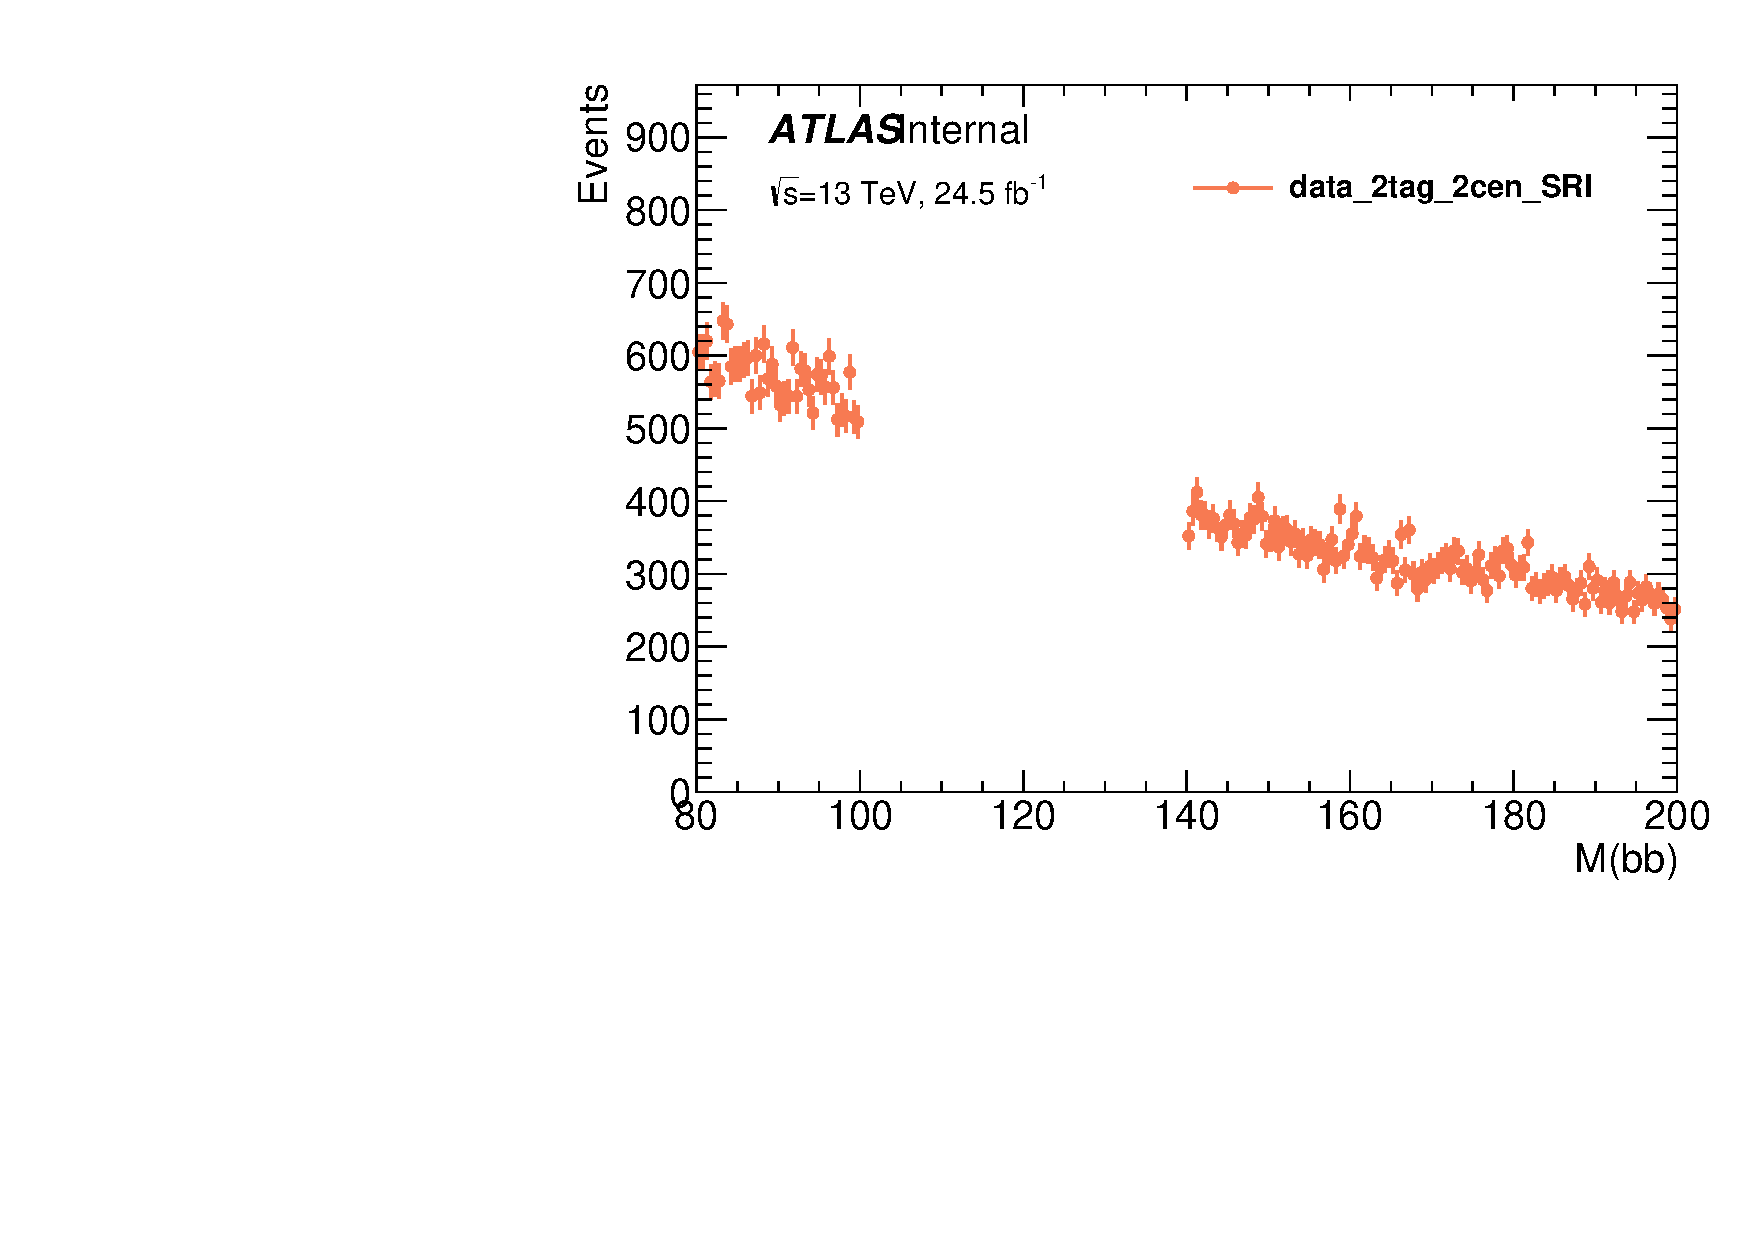
\includegraphics[width=0.45\textwidth]{figures_alt/Mbb_SRI_2cen.pdf}
 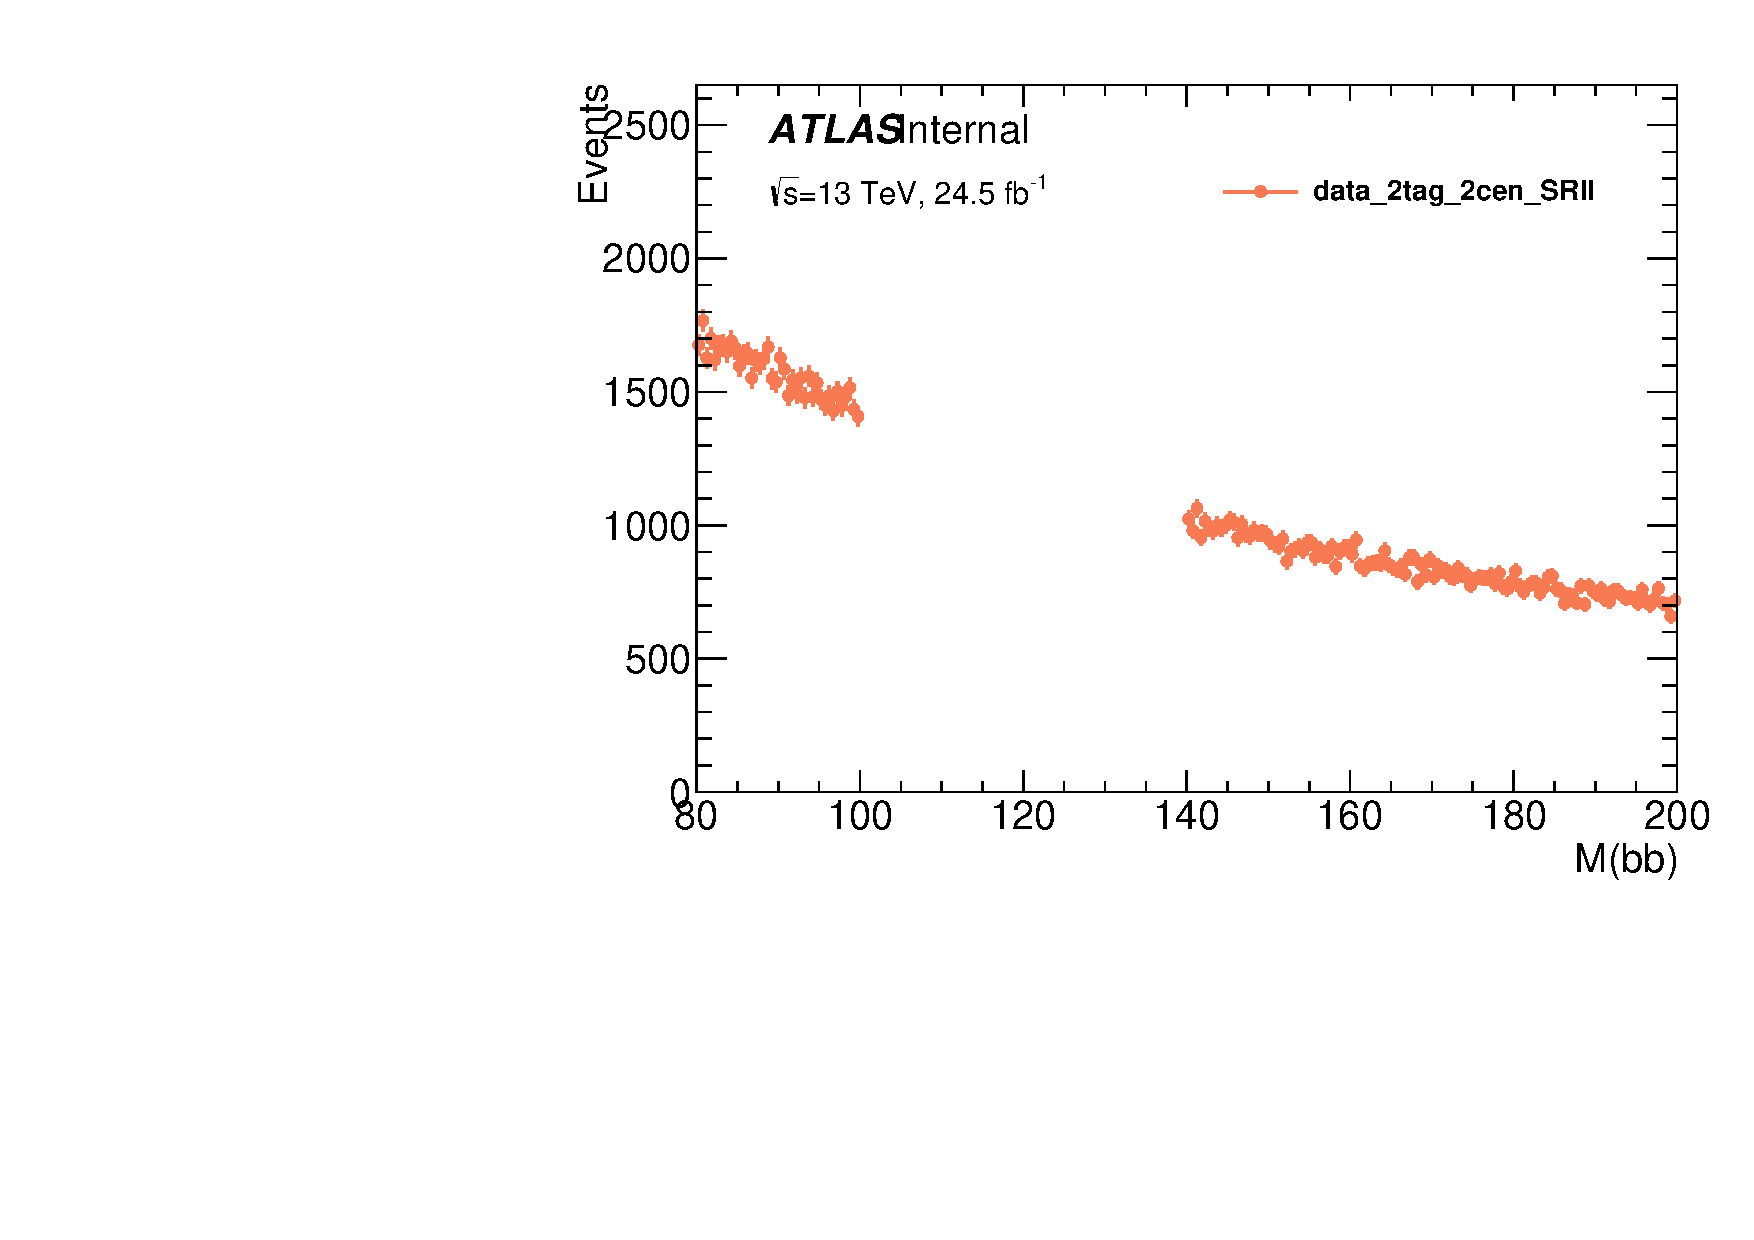
\includegraphics[width=0.45\textwidth]{figures_alt/Mbb_SRII_2cen.pdf}\\
 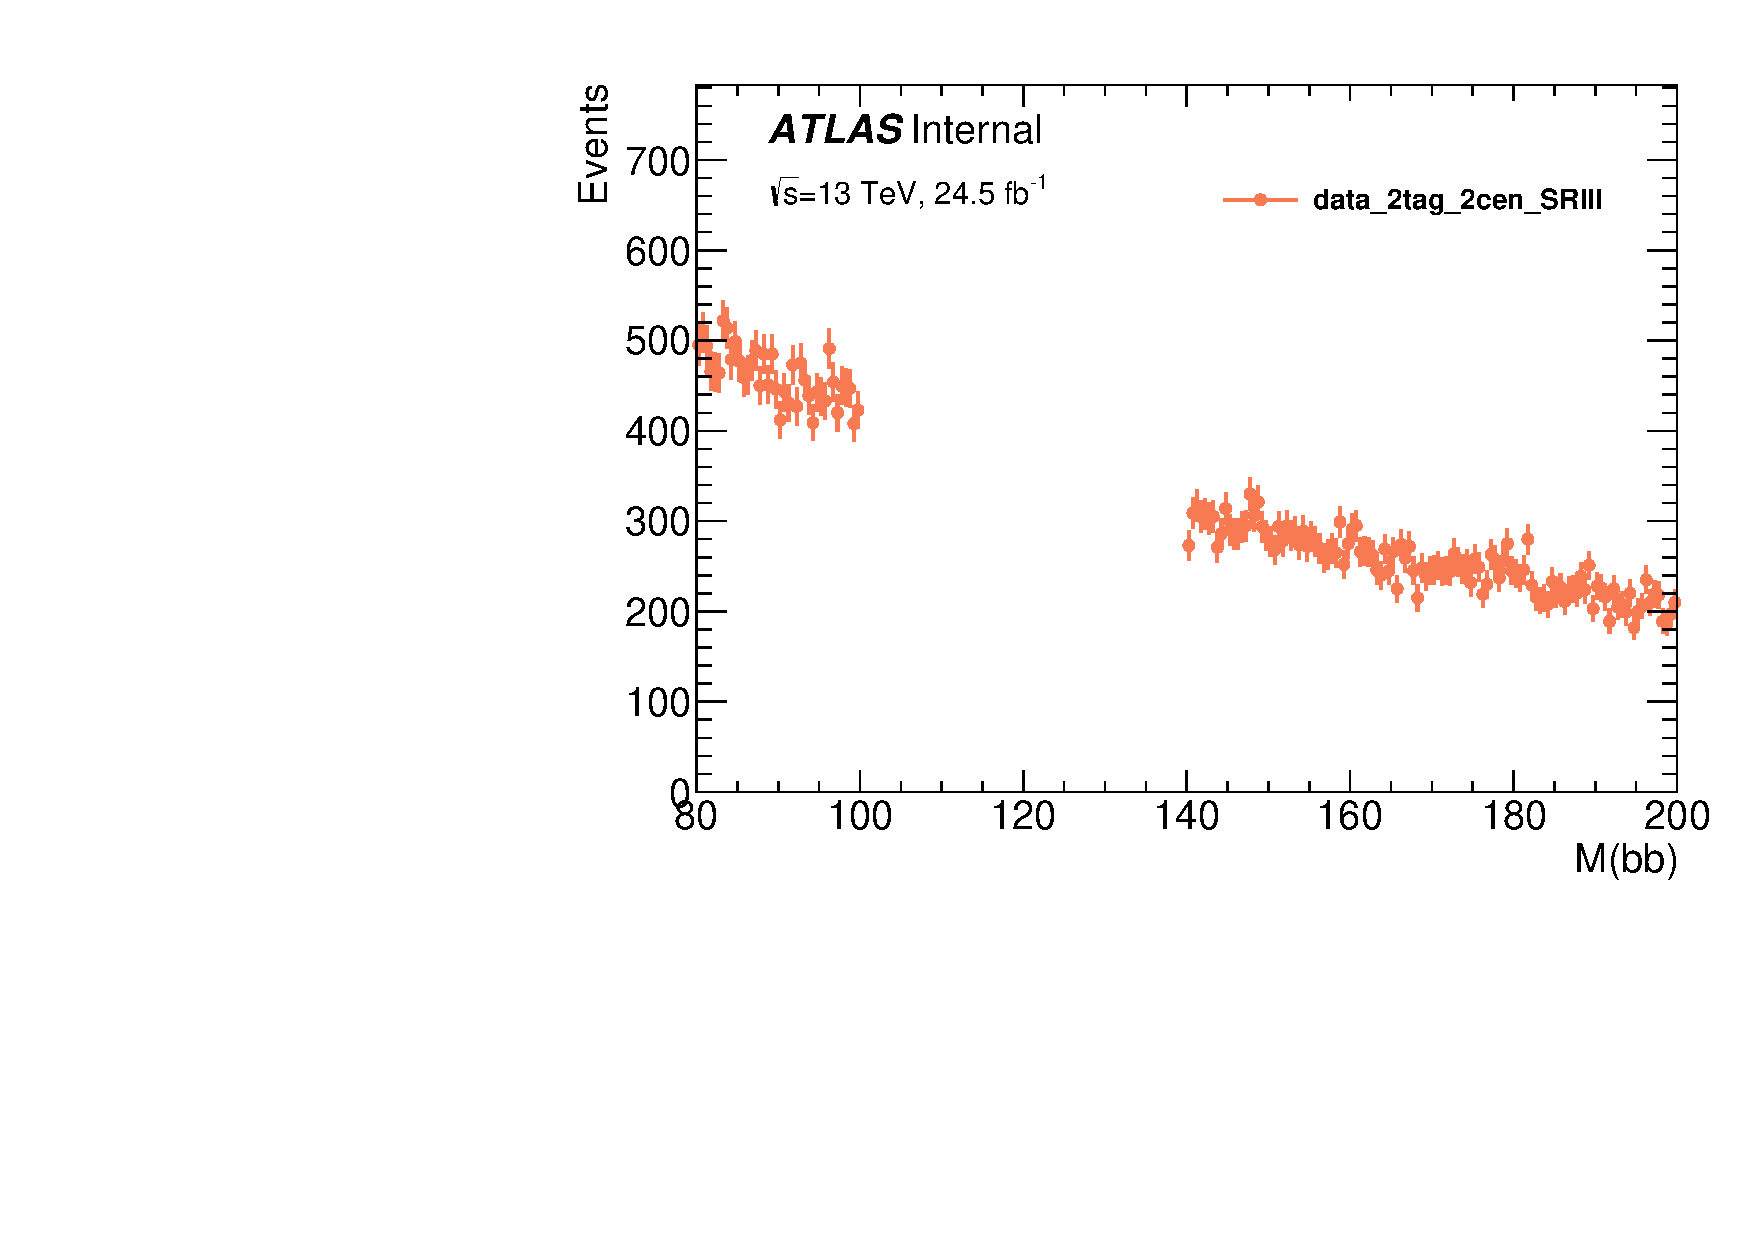
\includegraphics[width=0.45\textwidth]{figures_alt/Mbb_SRIII_2cen.pdf}
 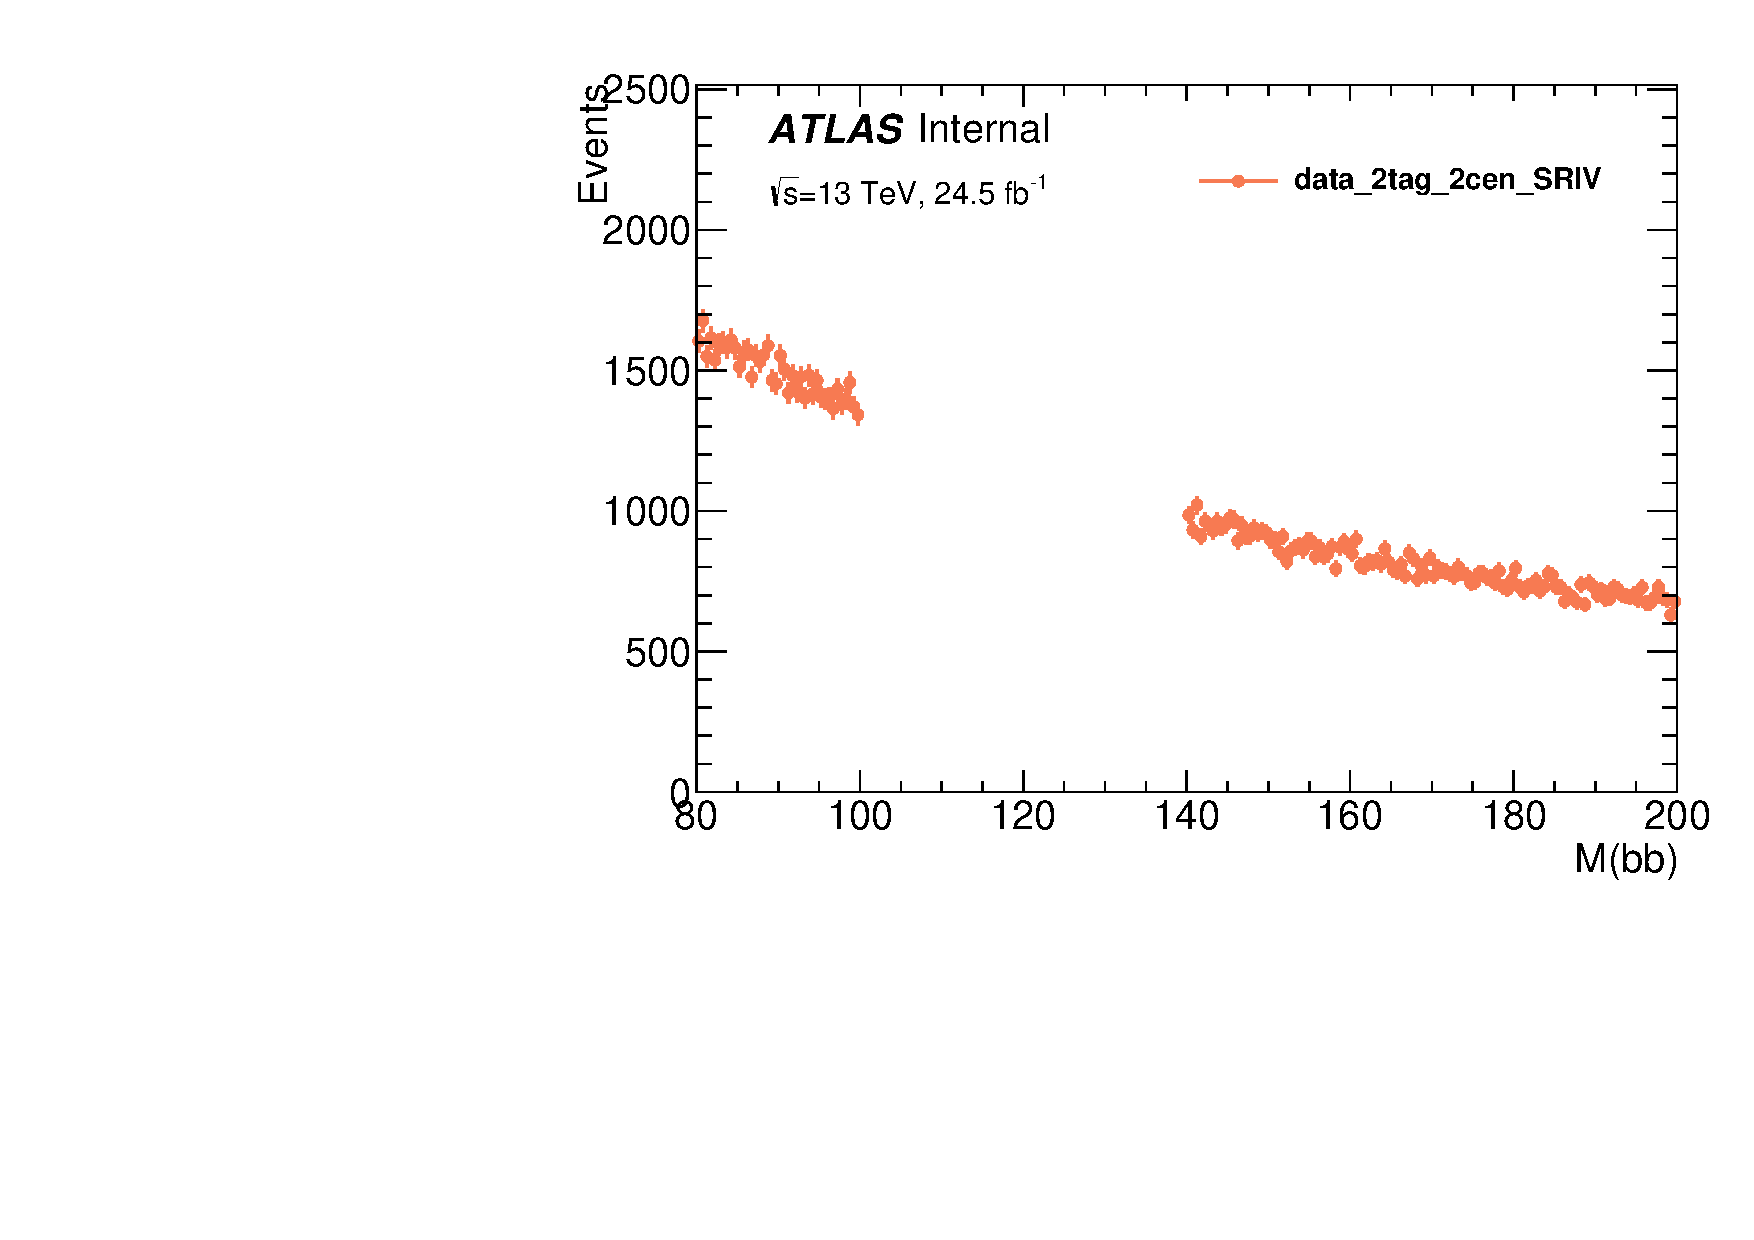
\includegraphics[width=0.45\textwidth]{figures_alt/Mbb_SRIV_2cen.pdf}\\
\caption{\Mbb{} shapes of BDT regions in sidebands} 
  \label{fig:mbb_sidebands_sensitive}
\end{figure}


\begin{table}[htbp]
\centering
\caption{Background only fit $\chi^2$ and Prob($\chi^2$) for \twocentral channel. The first number in each cell is the $\chi^2$ and the number in parentheses is the probability.}
\label{tab:chi2-2cen_sensitive}
\begin{tabular}{|l|l|l|l|l|l|l|}
\hline
   & \multicolumn{3}{c|}{\twocentral SR I}              & \multicolumn{3}{c|}{\twocentral SR II}             \\ \hline
   & Bernstein   & Expo*Bernstein & Sum of Expo & Bernstein   & Expo*Bernstein & Sum of Expo \\ \hline
O2 & 1.04 (0.37) & 1.06 (0.35)    & 1.04 (0.39)         & 1.16 (0.16) & 1.14 (0.19)    & 1.20 (0.12)         \\ \hline
O3 & 1.06 (0.35) & 0.98 (0.53)    & 1.01 (0.45)         & 1.12 (0.22) & 1.14 (0.19)    & 1.15 (0.17)         \\ \hline
O4 & 0.99 (0.50) & 0.99 (0.50)    & 1.01 (0.33)         & 1.12 (0.23) & 1.14 (0.19)    & 1.20 (0.11)         \\ \hline
O5 & 1.00 (0.49) &                &                     & 1.12 (0.23) &                &                     \\ \hline
   & \multicolumn{3}{c|}{\twocentral SR III}            & \multicolumn{3}{c|}{\twocentral SR IV}             \\ \hline
   & Bernstein   & Expo*Bernstein & Sum of Expo & Bernstein   & Expo*Bernstein & Sum of Expo \\ \hline
O2 & 1.12 (0.21) & 1.12 (0.22)    & 1.12 (0.22)         & 1.02 (0.42) & 0.99 (0.51)    & 0.98 (0.51)         \\ \hline
O3 & 1.11 (0.24) & 1.13 (0.21)    & 1.15 (0.17)         & 0.99 (0.50) & 1.00 (0.48)    & 1.03 (0.41)         \\ \hline
O4 & 1.12 (0.23) & 1.13 (0.21)    & 1.18 (0.14)         & 0.99 (0.51) & 1.00 (0.47)    & 1.04 (0.39)         \\ \hline
O5 & 1.15 (0.17) &                &                     & 0.99 (0.51) &                &                     \\ \hline
\end{tabular}
\end{table}


\begin{table}[htbp]
\centering
\caption{Value of the background only fit F-test for several sets of functions in \twocentral channel.}
\label{tab:f-test_sensitive}
\begin{tabular}{|l|l|l|l|l|}
\hline
Region               & SR I & SR II & SR III & SR IV \\ \hline
Bernstein O2/ O3     & 0.51 & 0.45  & 0.48   & 0.46  \\ \hline
Bernstein O3/ O4     & 0.44 & 0.51  & 0.50   & 0.50  \\ \hline
Bernstein O4/ O5     & 0.51 & 0.50  & 0.51   & 0.50  \\ \hline
Sum of Expo O2/O3    & 0.44 & 0.52  & 0.53   & 0.53  \\ \hline
Sum of Expo O3/O4    & 0.54 & 0.53  & 0.53   & 0.53  \\ \hline
Expo*Bernstein O2/O3 & 0.43 & 0.50  & 0.51   & 0.52  \\ \hline
Expo*Bernstein O3/O4 & 0.52 & 0.52  & 0.51   & 0.50  \\ \hline
\end{tabular}
\end{table}

\begin{table}[htbp]
\centering
\caption{Background spurious signal strength, $\mu_{\rm sp}$, in the spurious signal test for the \twocentral channel. The Bernstein functions ($f_B$) are tested against exponentials times Bernstein functions as well as the sum of exponentials ($f_A$).}
\label{tab:spurious-test-2cen_sensitive}
\begin{tabular}{|c|c|c|c|c|}
\hline
             & \multicolumn{2}{c|}{SR I}                  & \multicolumn{2}{c|}{SR II}                 \\ \hline
             & Expo*Bernstein O2 & Sum of Expo O2 & Expo*Bernstein O2 & Sum of Expo O2 \\ \hline
Bernstein O2 & \textless0.01     & 0.48                   & 6.1               & 2.8                    \\ \hline
Bernstein O3 & \textless0.01     & 0.02                   & 0.33              & 0.05                   \\ \hline
             & \multicolumn{2}{c|}{SR III}                & \multicolumn{2}{c|}{SR IV}                 \\ \hline
             & Expo*Bernstein O2 & Sum of Expo O2 & Expo*Bernstein O2 & Sum of Expo O2 \\ \hline
Bernstein O2 & 1.9               & 2.3                    & 10.2              & 10.7                   \\ \hline
Bernstein O3 & 0.32              & 0.03                   & 0.06              & 0.08                   \\ \hline
\end{tabular}
\end{table}


\begin{figure}[htbp]
  \centering
 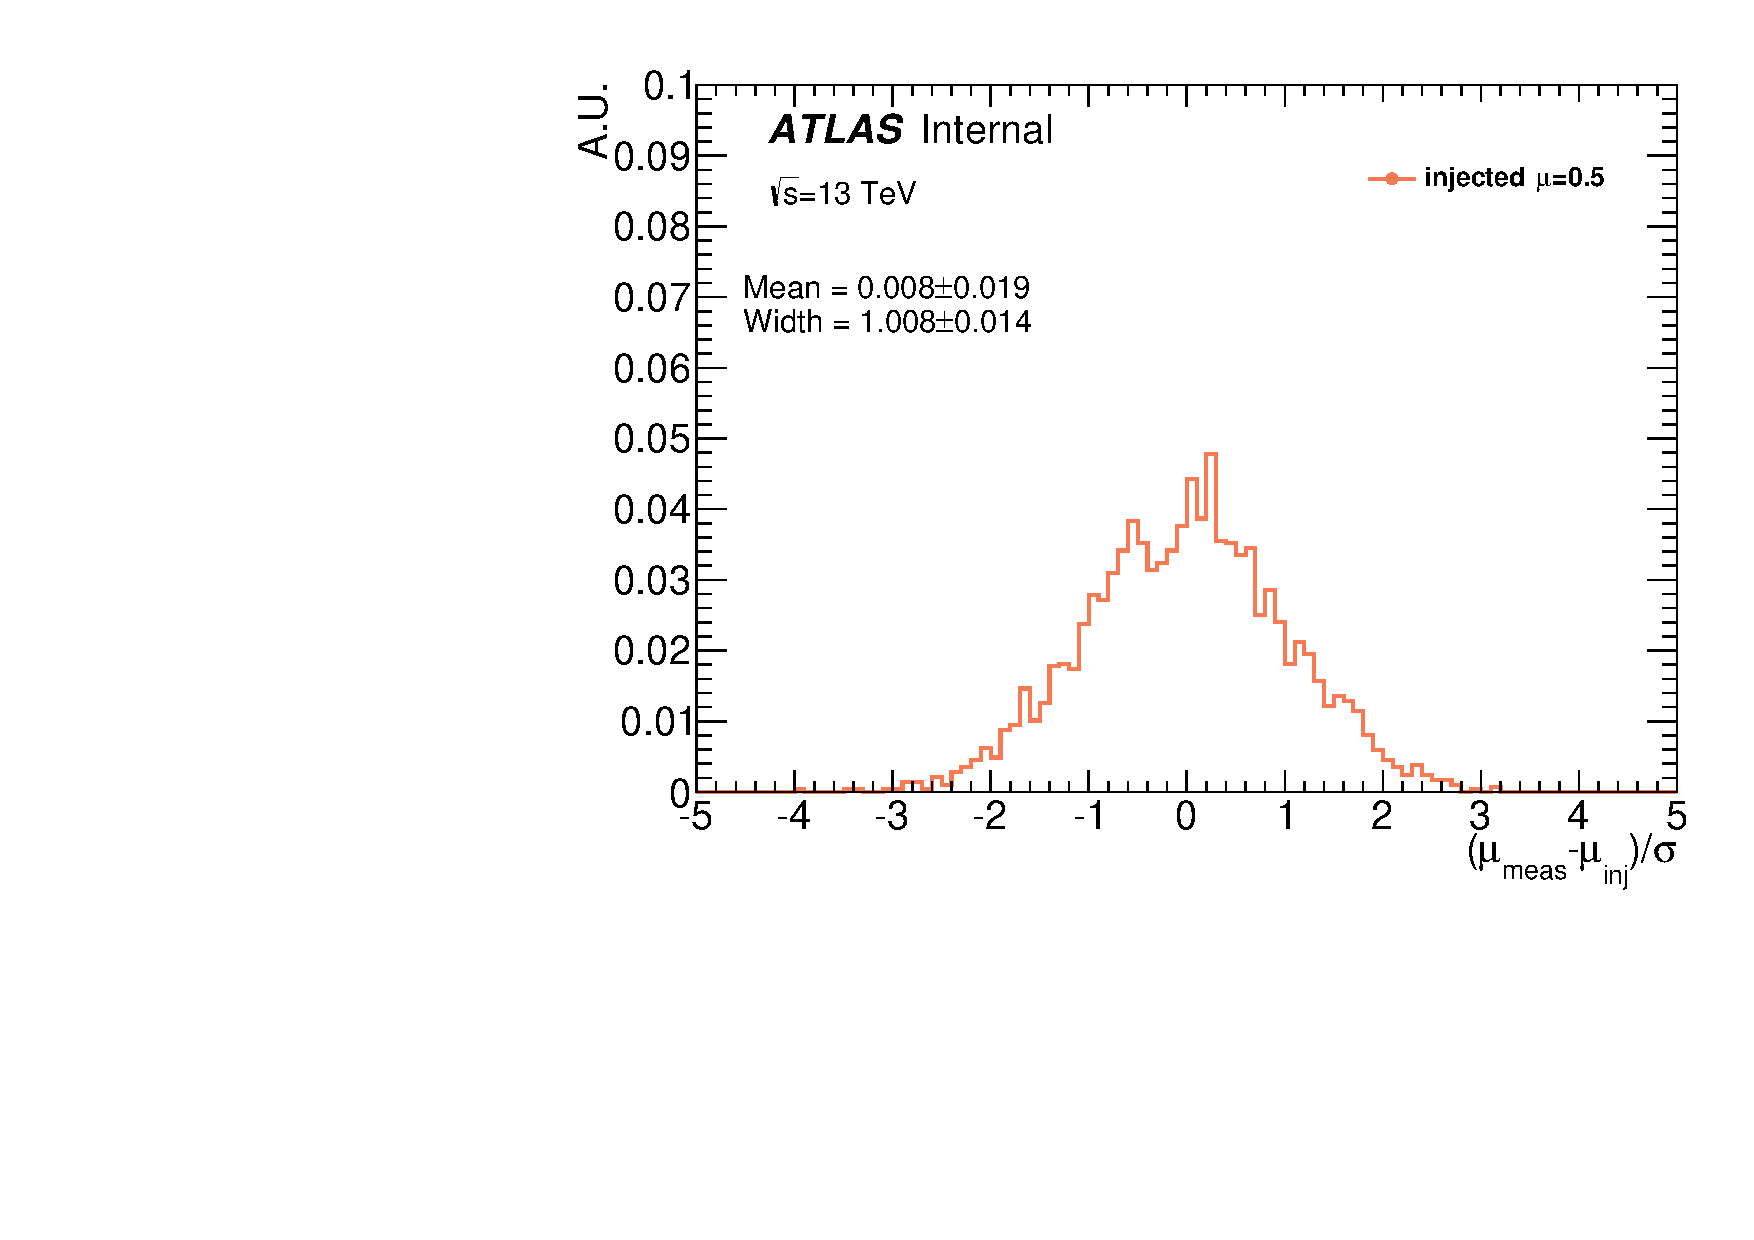
\includegraphics[width=0.45\textwidth]{figures_alt/Mu05.pdf}
 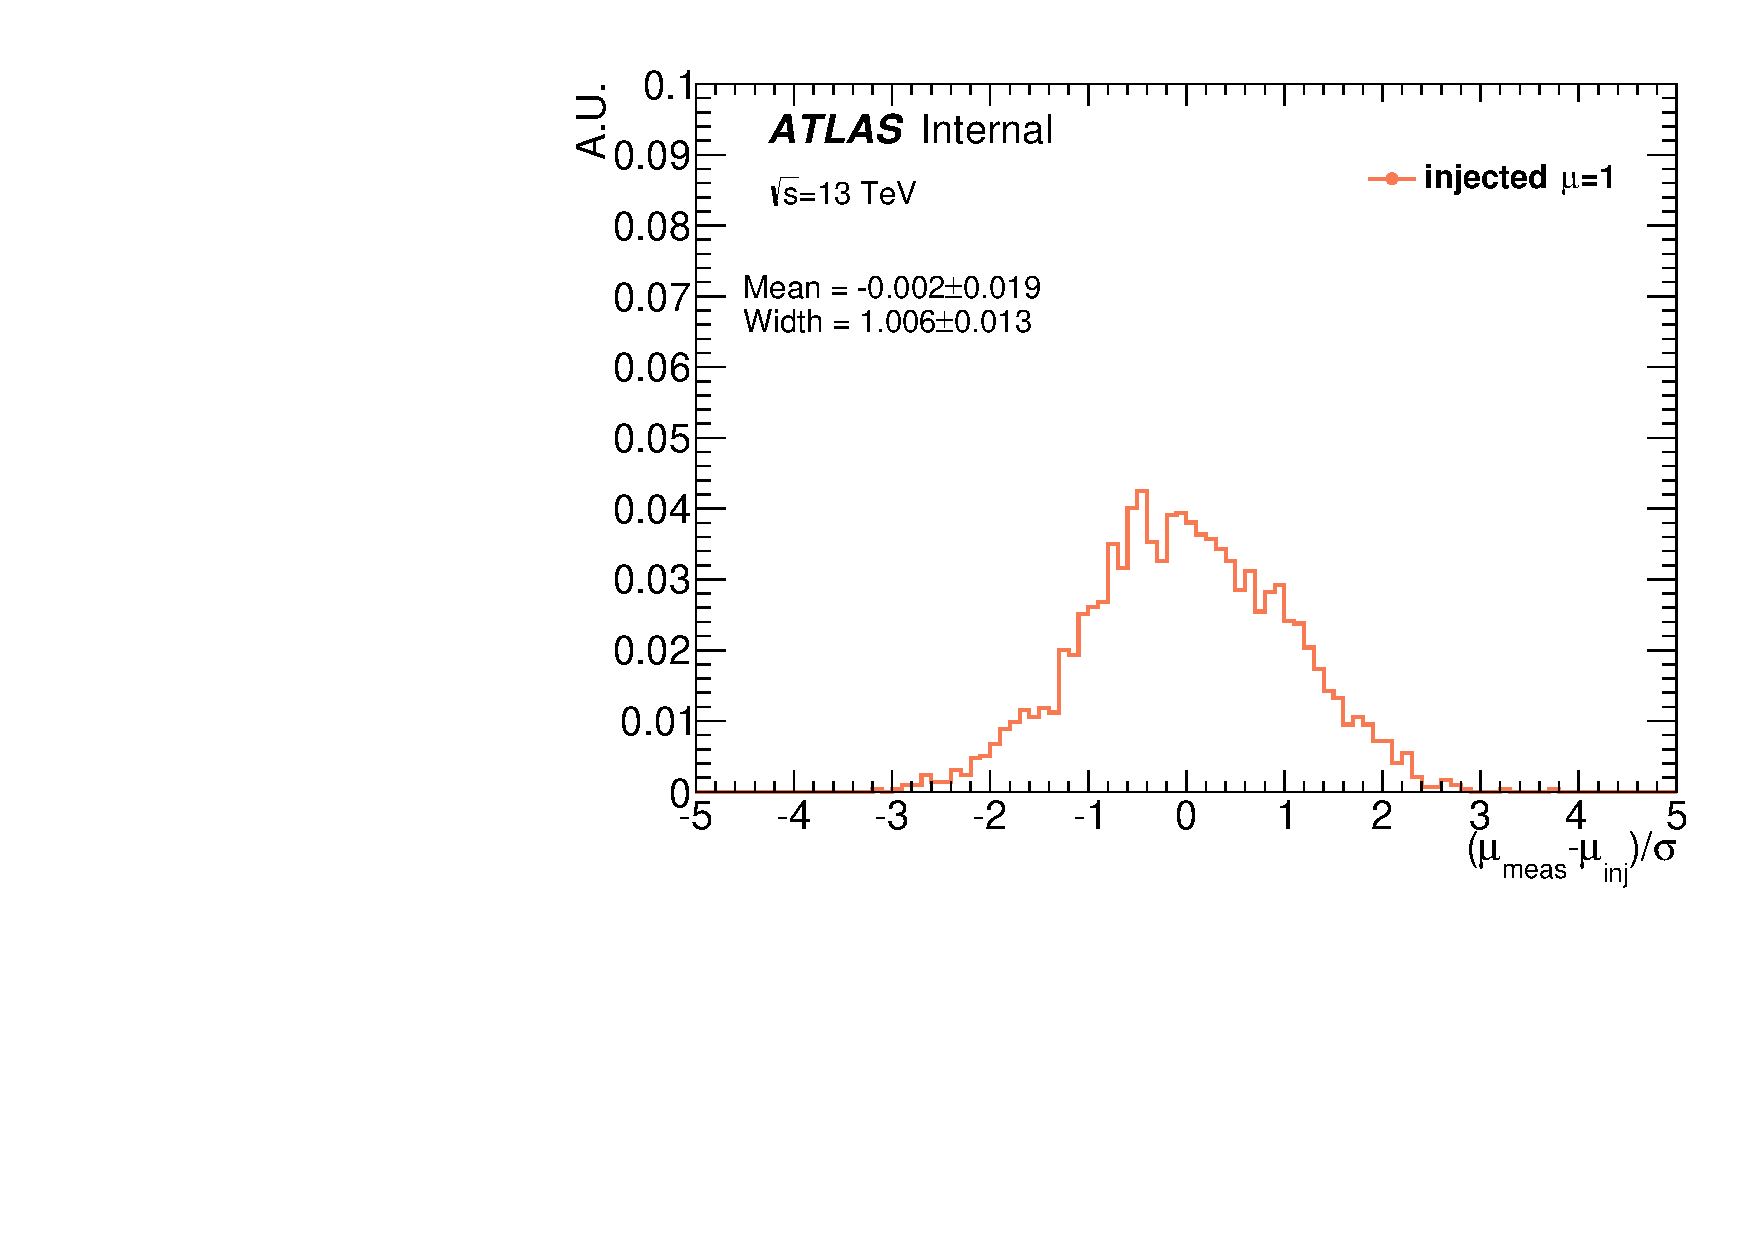
\includegraphics[width=0.45\textwidth]{figures_alt/Mu1.pdf}\\
 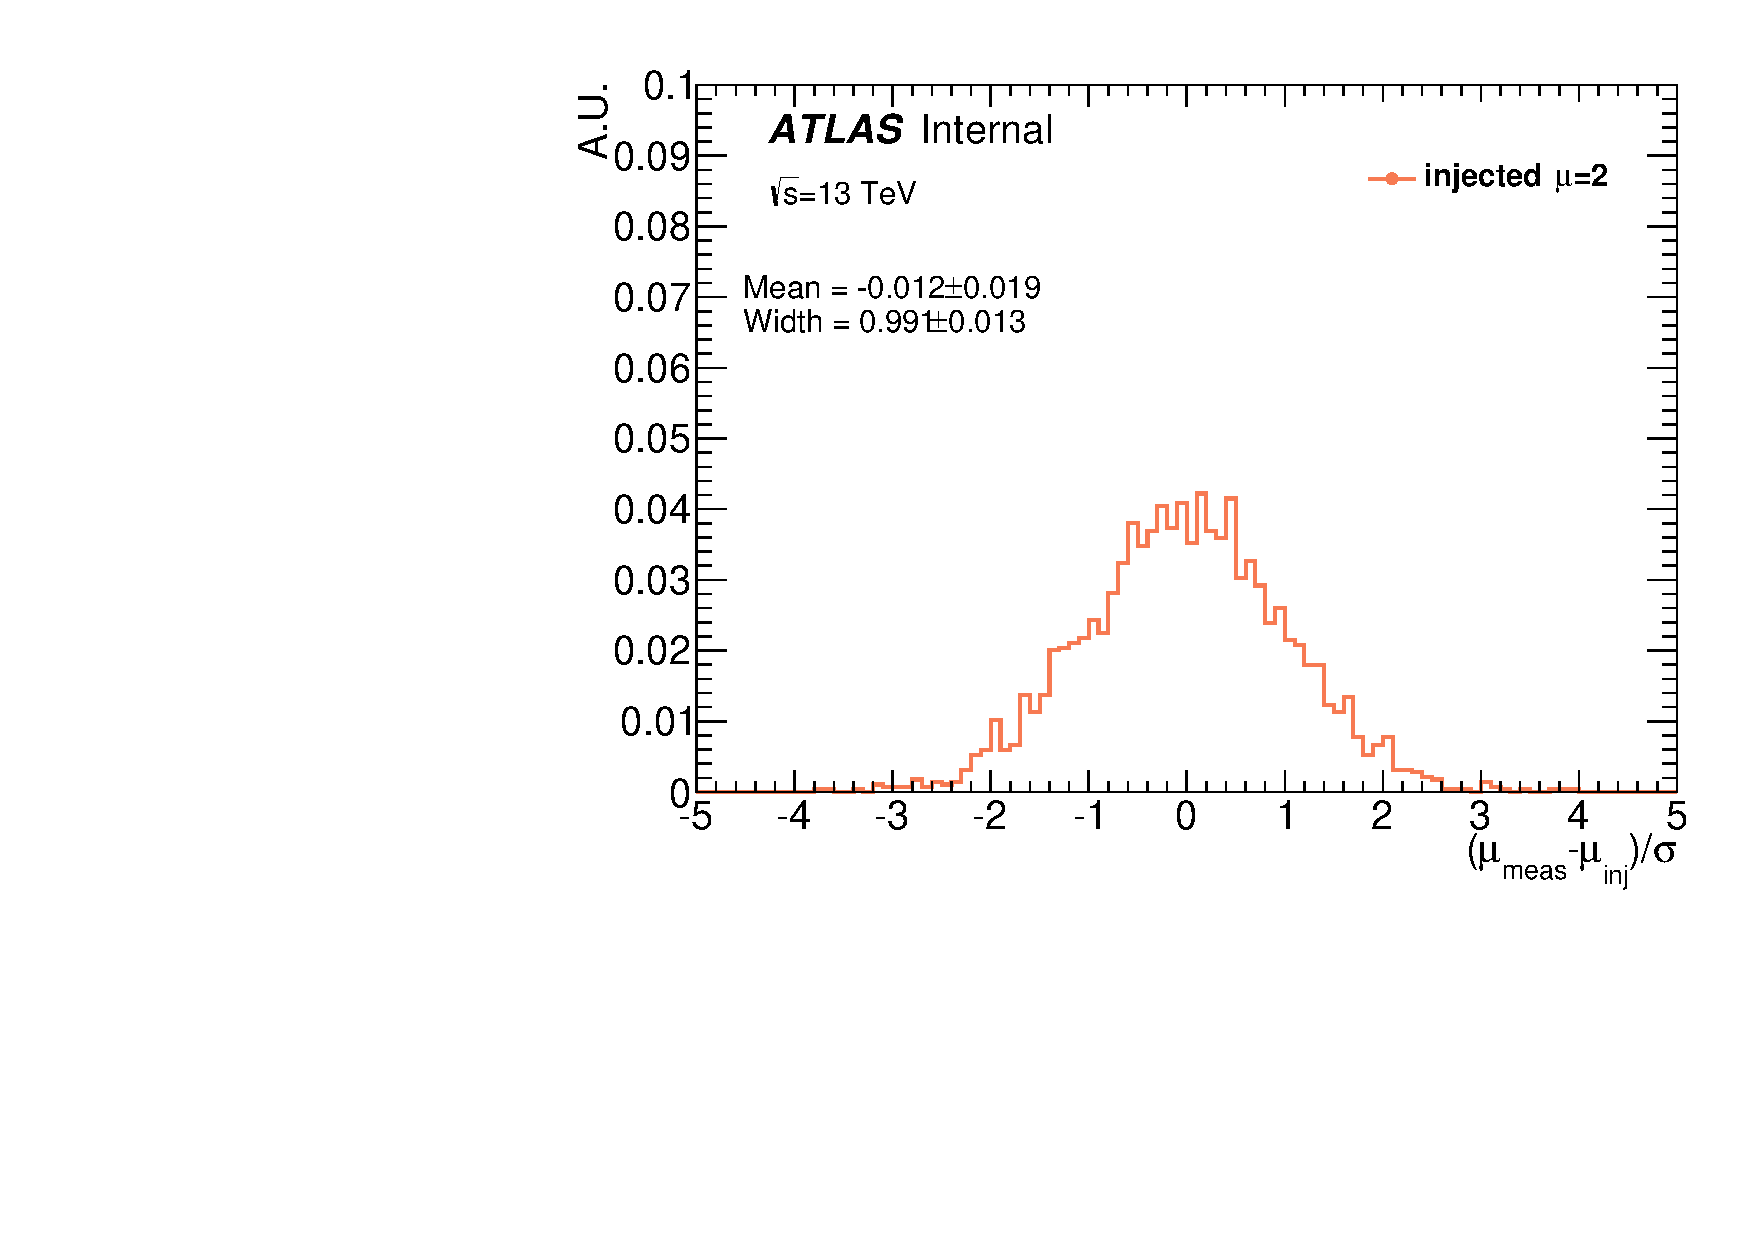
\includegraphics[width=0.45\textwidth]{figures_alt/Mu2.pdf}
 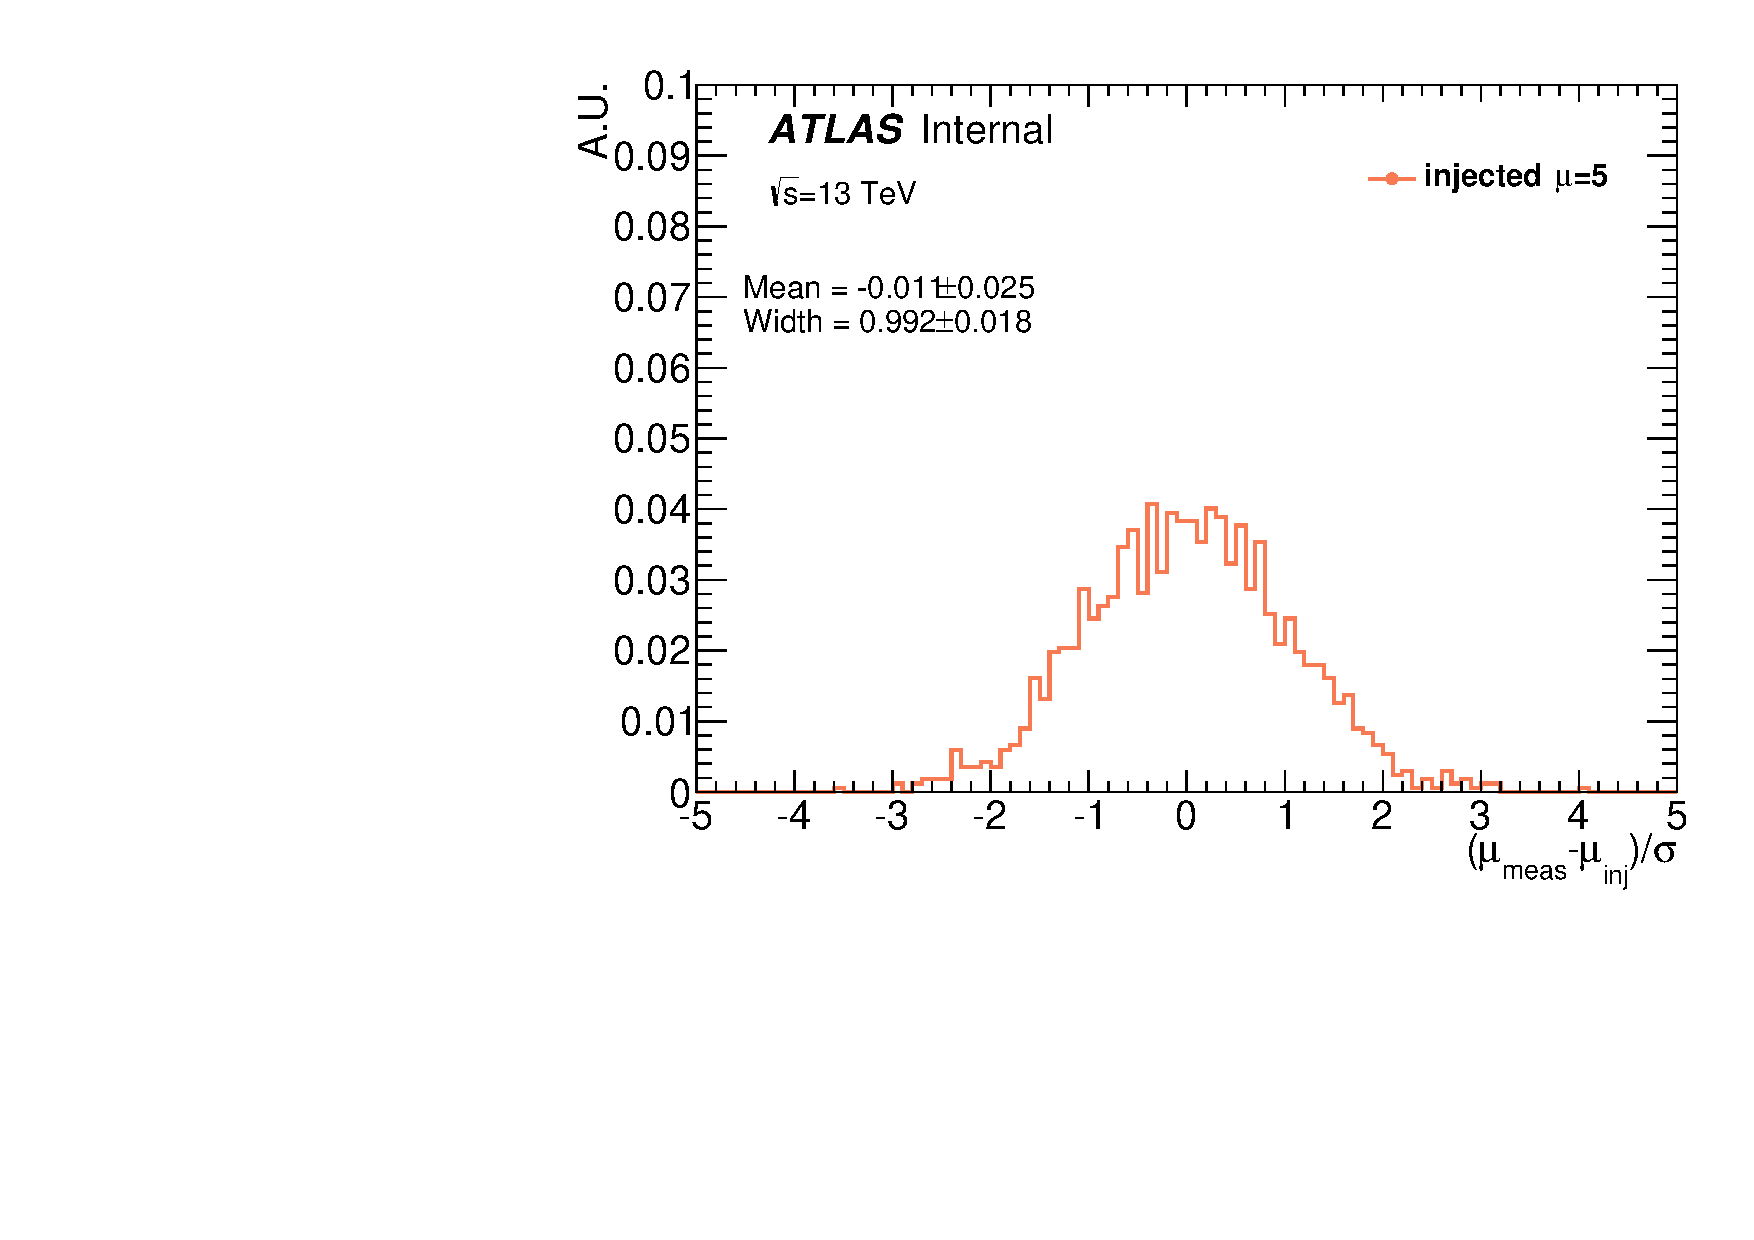
\includegraphics[width=0.45\textwidth]{figures_alt/Mu5.pdf}\\
\caption{Pull distribution of toy experiment fits. We inject Higgs signal strength of 0.5 (top left), 1.0 (top right), 2.0 (bottom left) and 5.0 (bottom right) times the Standard Model prediction. The pulls are fitted with Gaussian to determine the means and widths which are unbiased. }
  \label{fig:MCToy_sensitive}
\end{figure}


\begin{table}[htbp]
\centering
\caption{Floating Z normalization parameters in Asimov fit}
\label{tab:zstrength_sensitive}
\begin{tabular}{|c|c|}
\hline
Region               & Asimov fit Z signal strength \\ \hline
SR I, \twocentral    & $ 1.00 \pm 3.2$              \\ \hline
SR II, \twocentral   & $ 1.00 \pm 1.78$             \\ \hline
SR III, \twocentral  & $ 1.00 \pm 0.79$             \\ \hline
SR IV, \twocentral   & $ 1.00 \pm 0.49$             \\ \hline
SR I, \fourcentral   & $ 1.00 \pm 1.13$             \\ \hline
SR II, \fourcentral  & $ 1.00 \pm 0.66$             \\ \hline
SR III, \fourcentral & $ 1.00 \pm 0.36$             \\ \hline
SR IV, \fourcentral  & $ 1.00 \pm 0.21$             \\ \hline
\end{tabular}
\end{table}


\begin{table}[htbp]
\centering
\caption{Floating Z normalization parameters in data sideband fit}
\label{tab:zsidebandfit_sensitive}
\begin{tabular}{|l|c|c|}
\hline
Channel      & $\mu_{Z}$   & $\chi^2/ndof$ \\ \hline
2 cen SR I   & 15.87±5.23 & 0.87          \\ \hline
2 cen SR II  & 4.56±2.88  & 1.01          \\ \hline
2 cen SR III & 0.96±1.28  & 0.92          \\ \hline
2 cen SR IV  & 0.33±0.85  & 0.85          \\ \hline
4 cen SR I   & 2.18±1.98  & 0.82          \\ \hline
4 cen SR II  & 2.00±1.93  & 0.89          \\ \hline
4 cen SR III & 1.90±0.63  & 0.92          \\ \hline
4 cen SR IV  & 0.56±0.55  & 0.91          \\ \hline
\end{tabular}
\end{table}


\begin{figure}[htbp]
  \centering
 \includegraphics[width=0.9\textwidth]{figures_final/Zfit_2cen_overlay_Nominal.PNG}
\caption{Overlay of sideband only fit fully floating the $\mu_{Z}$ contribution and fixing $\mu_{Z}=1$ in $\twocentral$ channel for the main analysis BDT region definition. The non-resonant background function overlap with each other within the uncertainty.}
  \label{fig:2cen_overlay}
\end{figure}

\begin{figure}[htbp]
  \centering
 \includegraphics[width=0.9\textwidth]{figures_final/Zfit_4cen_overlay_Nominal.PNG}
\caption{Overlay of sideband only fit fully floating the $\mu_{Z}$ contribution and fixing $\mu_{Z}=1$ in $\fourcentral$ channel for the main analysis BDT region definition. The non-resonant background function overlap with each other within the uncertainty.}
  \label{fig:4cen_overlay}
\end{figure}


\begin{figure}[htbp]
  \centering
 \includegraphics[width=0.6\textwidth]{figures_alt/Zfit_2cen_overlay.PNG}
\caption{Overlay of sideband only fit fully floating the $\mu_{Z}$ contribution and fixing $\mu_{Z}=2$ in $\twocentral$ channel SR I for the alternative and aggressive BDT region definition. The upper sideband has no impact constraining the lower sideband and the \zjets{} contribution.}
  \label{fig:SRI_overlay_sensitive}
\end{figure}

